%!TEX root = ../../../report.tex
\section{Joints} % (fold)
\label{sec:joints}

\begin{figure}[ht!]
  \centering
  \includegraphics[width=\textwidth]{figures/20160518_195014.jpg}
  \caption{Might help}
  \label{fig:figure1}
\end{figure}

  \subsection{Actuators} % (fold)
  \label{sub:actuators}

  % subsection actuators (end)

  \subsection{Transmission} % (fold)
  \label{sub:transmission}

  % subsection transmission (end)

  \subsection{Compliance} % (fold)
  \label{sub:compliance}


  \begin{figure}[hb!]
    \begin{subfigure}{.19\textwidth}
      \centering
      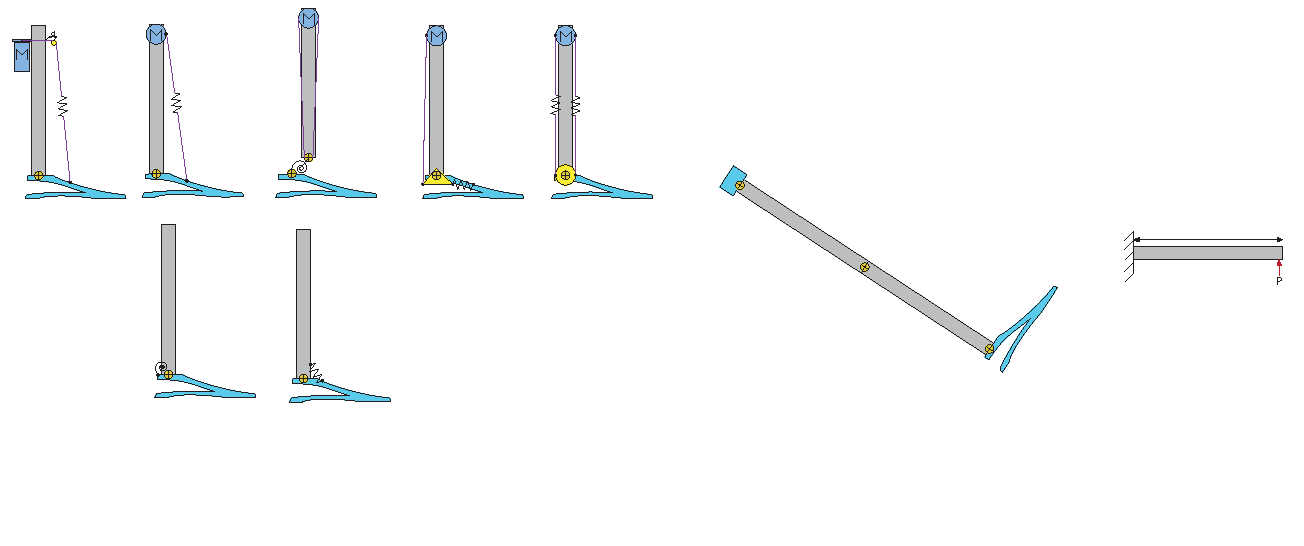
\includegraphics[width=\linewidth]{figures/illustration_serial_pulley.pdf}
      \caption{Serial pulley}
      \label{fig:series_pulley}
    \end{subfigure}
    \begin{subfigure}{.19\textwidth}
      \centering
      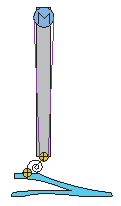
\includegraphics[width=\linewidth]{figures/illustration_serial_rotational.pdf}
      \caption{Series rotational}
      \label{fig:series_rotational}
    \end{subfigure}
    \begin{subfigure}{.19\textwidth}
      \centering
      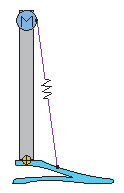
\includegraphics[width=\linewidth]{figures/illustration_serial_direct_i.pdf}
      \caption{Series direct 1}
      \label{fig:series_direct_i}
    \end{subfigure}
    \begin{subfigure}{.19\textwidth}
      \centering
      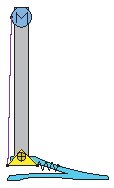
\includegraphics[width=\linewidth]{figures/illustration_serial_direct_ii.pdf}
      \caption{Series direct 2}
      \label{fig:series_direct_ii}
    \end{subfigure}
    \begin{subfigure}{.19\textwidth}
      \centering
      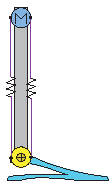
\includegraphics[width=\linewidth]{figures/illustration_serial_elastic_band.pdf}
      \caption{Series elastic band}
      \label{fig:series_elastic_band}
    \end{subfigure}
  \end{figure}  

  % subsection compliance (end)

% section joints (end)